%%%%%%%%%%%%%%%%%%%%%%%%%
% Dokumentinformationen %
%%%%%%%%%%%%%%%%%%%%%%%%%
%
% (c) 2013 Lukas Loser und Dorian Amiet
%
 
%%%%%%%%%%%%%%%%%%%%%%%%%%%%%%%%%%%%%%%%%%%%%
% Standard projektübergreifender Header für 
% - Makros 
% - Farben
% - Mathematische Operatoren
%
% DORT NUR ERGÄNZEN, NICHTS LÖSCHEN
%%%%%%%%%%%%%%%%%%%%%%%%%%%%%%%%%%%%%%%%%%%%%

\chapter{Das Innere-Punkte-Verfahren}
\rhead{Das Innere-Punkte-Verfahren}

\chapterauthor{Dorian Amiet und Lukas Loser}
\begin{refsection}

\section{Einleitung}
Innere-Punkte-Verfahren sind Algorithmen f"ur die Optimierung von linearen
und quadratischen Programmen \cite{ip:wiki}, \cite{ip:tunc}, \cite{ip:werner}.
Im Vergleich beispielsweise zum Simplex-Verfahren
zeichnet sich das Innere-Punkte-Verfahren durch schnellere Konvergenz
bei d"unn besetzten Problemen aus. Im Gegensatz zum Simplex Algorithmus, der
den Kanten folgt, geht das Innere-Punkte Verfahren den
inneren Punkten nach bis zum Optimum (respektive zu dem Ort mit einer
gen"ugend kleinen Abweichung), symbolisiert in der nachstehenden Abblidung
durch den roten Pfad.
\begin{center}
  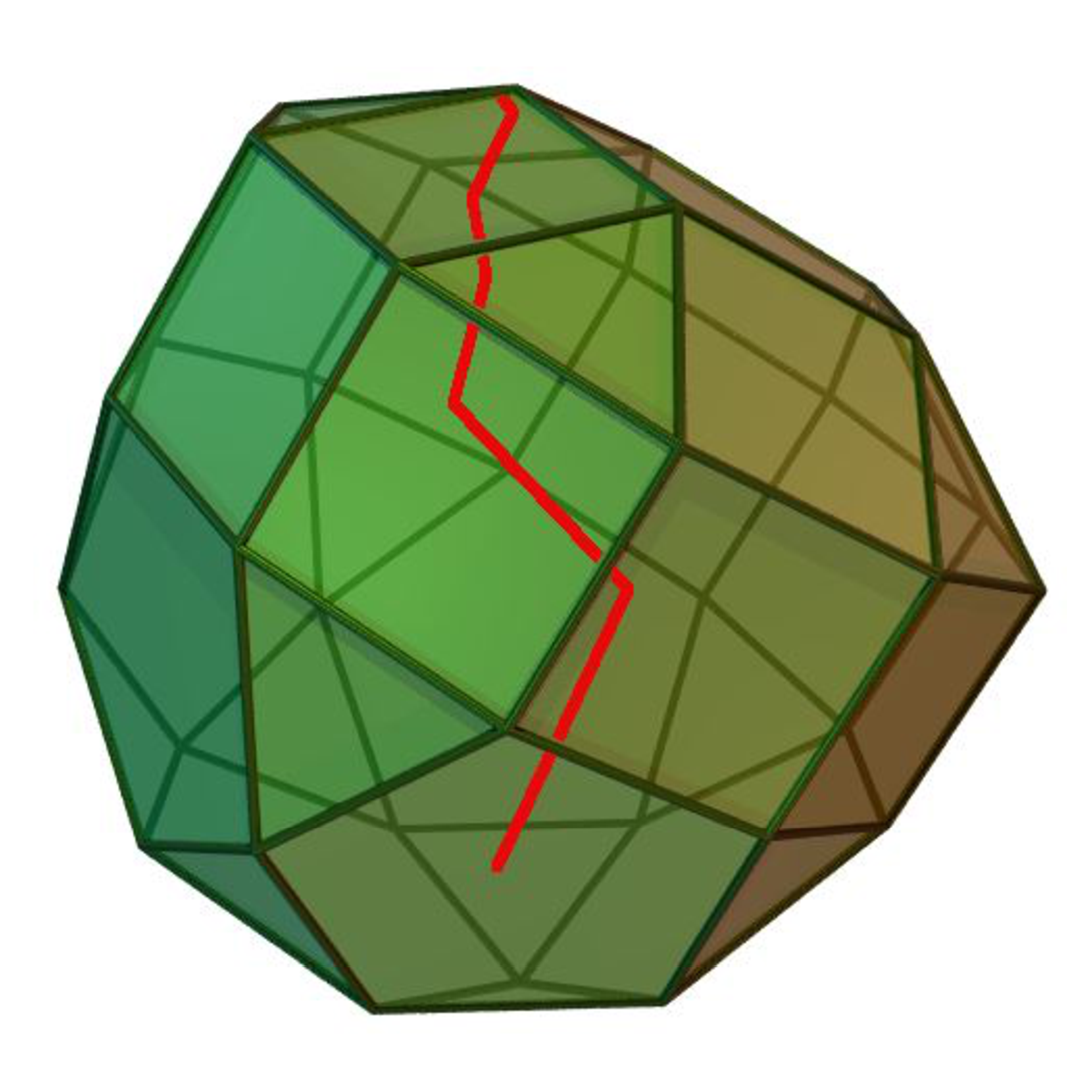
\includegraphics[scale=0.3]{innerepunkte/Interior-point-method-three-dimensions.pdf}
\end{center}
	
	
\section{Idee der Strafterme}
Vielfach gibt es f"ur den zu optimierenden Vektor $x$ eine untere und
eine obere Grenze ({\tt lb}, {\tt ub}) als Nebenbedingung.
Damit diese Nebenbedingung nicht
verletzt wird, braucht es ein Strafverfahren und das funktioniert so:
\begin{quotation}
\parindent 0pt
Bestrafe die Verletzung der Nebenbedingung in der Zielfunktion mit einem
Strafterm, der mit
einem Strafparameter gewichtet wird, und l"ose eine Folge mit dieser
Zielfunktion
f"ur wachsenden Strafparameter, bis die Verletzung klein genug ist.
\end{quotation}
Der {\it Strafterm} soll sich bei der Suche nach einem Minimum extrem
vergr"ossern, sobald sich $x$ dem Grenzwert $x \to x_0$ ann"ahert.
Daher verwendet man als Strafterm oft:
\[
\mu \cdot \log(x-x_0)
\]
Der Term
$-\log(x)$ strebt f"ur $x\to 0+$ gegen unendlich.
Addiert man einen Term $-\mu\log(x-x_0)$
zur Zielfunktion eines Minimumproblems,
wird die Zielfunktion in der N"ahe von $x_0$ extrem gross,
jeder Algorithmus, der Minima finden kann, wird dem Punkt $x_0$
fern bleiben, selbst wenn dort das Minimum des urspr"unglichen
Problems ist. Stattdessen wird der Algorithmus eine L"osung in
der N"ahe von $x_0$ finden.

Wenn man allerdings den Wert von $\mu$ verringert, wird der
Einfluss des Strafterms kleiner. Ist $x_0$ die L"osung des
urspr"unglichen Minimalproblems, wird die L"osung des Minimalproblems
mit Strafterm $-\mu\log(x-x_0)$ je n"aher an $x_0$ heranr"ucken,
je kleiner $\mu$ gemacht wird.

Die Strafterme
werden in der Octave-Funktion automatisch verarbeitet. Es m"ussen nur die
Grenzen als Vektoren angegeben werden (${\tt lb}= \text{lower bound}$,
${\tt ub} = \text{upper bound}$)

Je kleiner $\mu$ gew"ahlt wird, desto kleiner wird der Fehler durch die
Strafterme, ausgenommen wenn x an die Grenzen kommt $x \to x_0$, dann
geht $f \to \infty$. F"ur $\mu \to 0$ resultiert die Zielfunktion
mit Ausnahme der zwei Extremalstellen bei $x=2$ und $x=4$. Jetzt muss
also nur noch daf"ur gesorgt werden, dass der Punkt X zu Beginn zwischen
den Barrieren liegt!

F"ur ein lineares Optimierungsproblem mit Zielfunktion $c^t\cdot x$ 
und Nebenbedingungen $x_i\ge x_{i0}$ werden Strafterme f"ur jede
der Nebenbedingungen hinzugef"ugt:
\[
 \operatorname{min}\biggl(c^t \cdot x - \mu \cdot \sum_{i=1}^n{\log(x_i -
x_{i0})}\biggr)\qquad
\text{und}\qquad    \operatorname{max}\biggl(c^t \cdot x + \mu \cdot \sum_{i=1}^n{\log(x_i
- x_{i0})}\biggr)
\]

{\parindent 0pt \bf Beispiel:} Suche das Minimum der Funktion $f=x^2-2x$ mit den
Grenzen $x\in[2,4]$. Die mit Straftermen modifizierte Zielfunktion ist
in Abbildung \ref{innerepunkte:strafterme} und \ref{innerpunkte:strafterme2}
gezeigt.
Die modifizierte Zielfunktion hat ein lokales Minimum im Inneren
des Intervals.
Je kleiner $\mu$ gew"ahlt wird, desto n"aher r"uckt
das lokale Minimum  zur gesuchten L"osung, n"amlich $x=2$.

\begin{figure}
\begin{minipage}[t]{6.0cm}
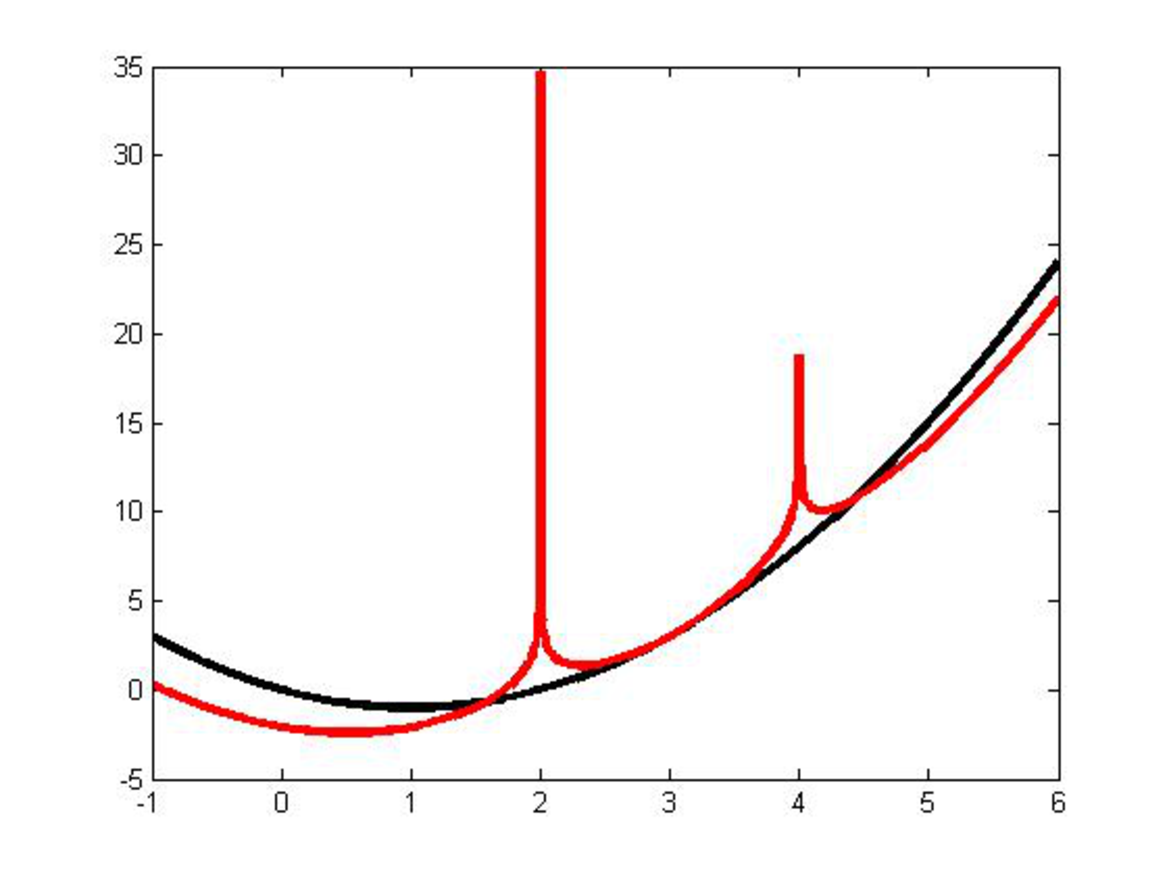
\includegraphics[width=6.0cm]{./innerepunkte/ln-barrieren-u=1.pdf}\\
	\end{minipage}
	\hspace{0.1cm}
	\begin{minipage}[t]{6.0cm}	
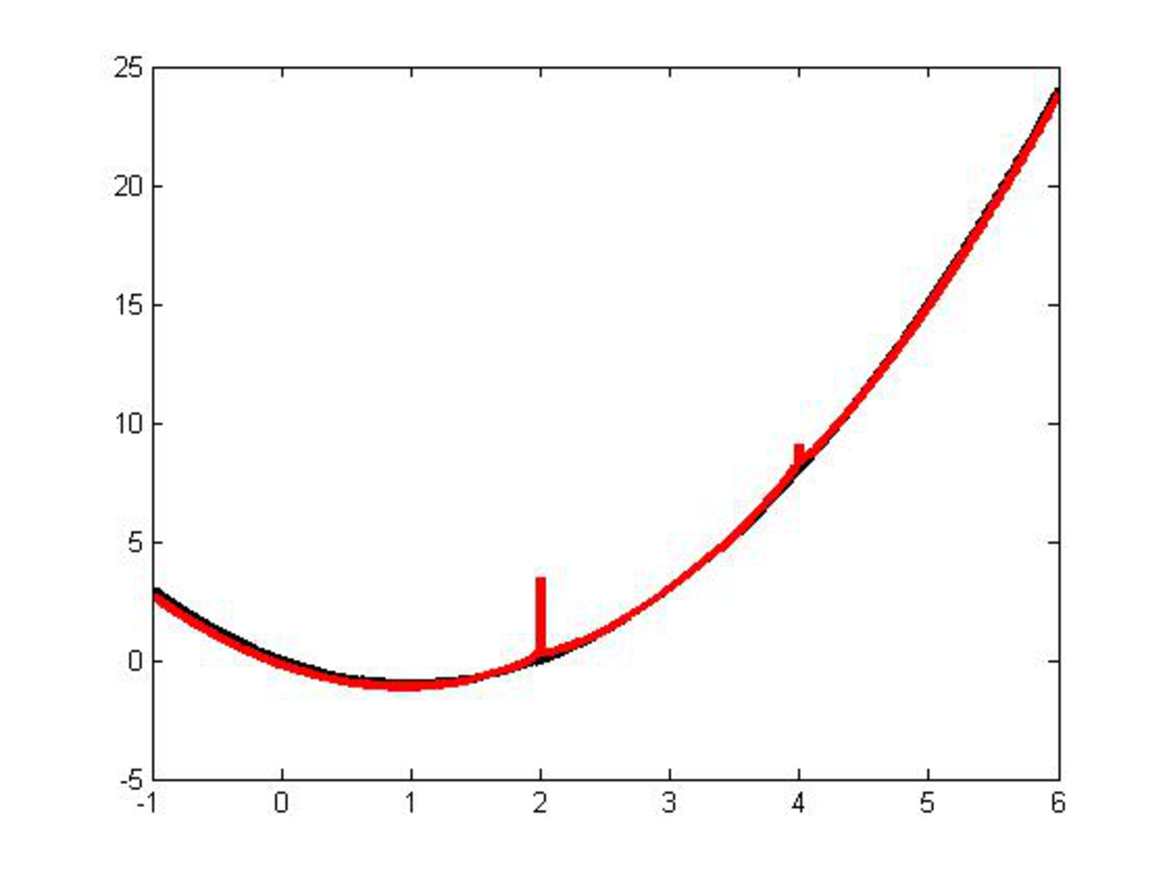
\includegraphics[width=6.0cm]{./innerepunkte/ln-barrieren-u=0_1-1.pdf}\\
	\end{minipage}
	\hspace{0.1cm}
	\begin{minipage}[t]{6.0cm}	
\end{minipage}
\caption{Auswirkung der Strafterme auf die Zielfunktion $f=x^2-2x$
f"ur $\mu=1$ (links) und $\mu=0.1$ (rechts).
\label{innerepunkte:strafterme}}
\end{figure}

\begin{figure}
\begin{center}
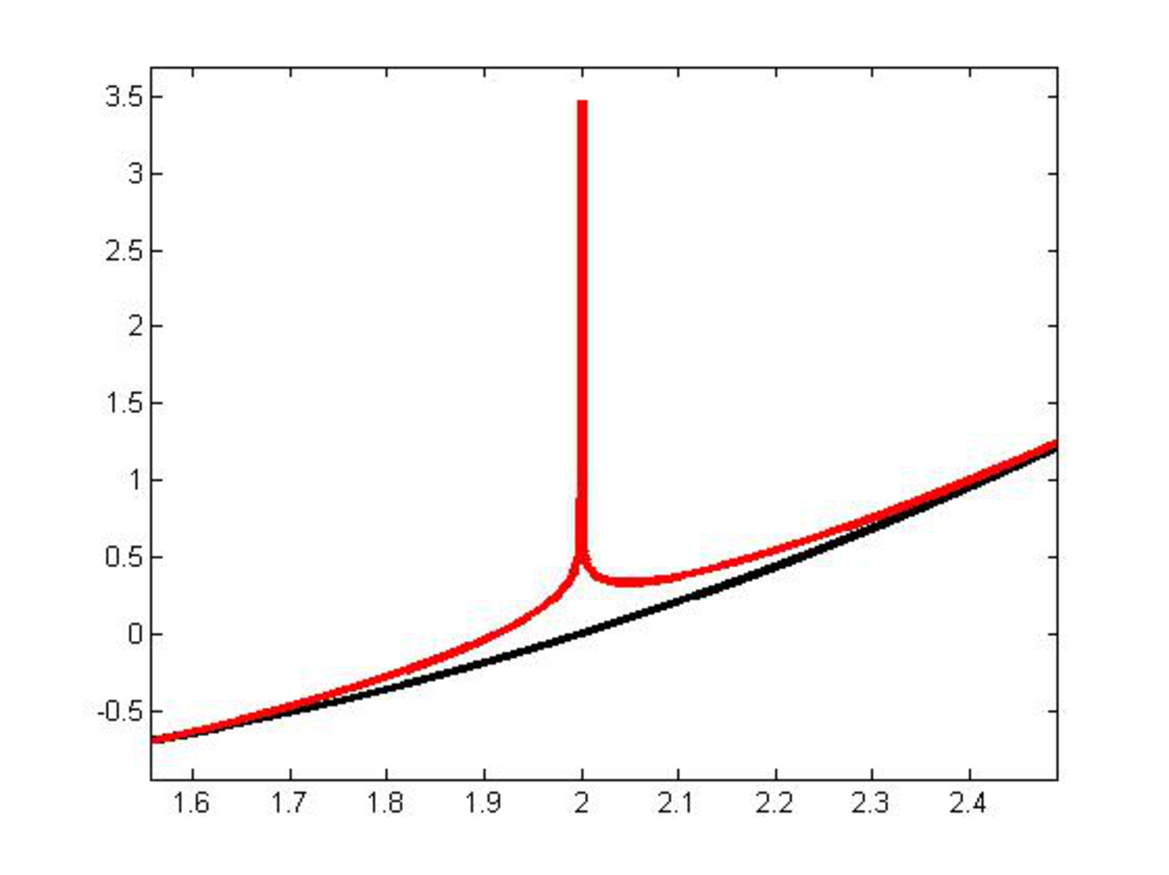
\includegraphics[width=6.0cm]{./innerepunkte/ln-barrieren-u=0_1-2.pdf}
\end{center}
\caption{Ausschnitt, $\mu=0.1$\label{innerpunkte:strafterme2}}
\end{figure}

\section{Der Algorithmus}
F"ur das Innere-Punkte-Verfahren gilt folgender, vereinfachter Algorithmus:

\begin{enumerate}
\item W"ahle primale und duale Startvektoren $\vec{x},\vec{y},\vec{s} > 0$\\
\begin{align*}
\vec{x}&= \text{Startvektor primales Problem}
\\
\vec{y}&=  \text{Startvektor duales Problem}
\\
\vec{s}&= \text{Startvektor Hilfsvariablen}
\end{align*}
\item Setze $\mu = \vec{x^t} \cdot \vec{s}/n$, darin ist
$\mu$ der Straftermparameter
\item Reduziere $\mu_{\text{neu}}=\mu_{\text{alt}} \cdot (1-\frac{\beta}{\sqrt{n}})$ mit $\beta \in ]0;0.5[$.
Man kann beweisen, dass der Algorithmus mit $\beta$ im genannten Intervall
immer konvergiert.
\item Berechne die Newton-Richtung durch L"osen des linearen Gleichungssystems
\[
\begin{bmatrix}
0 & A^t & I \\
A & 0 & 0 \\
S & 0 & X
\end{bmatrix}
\cdot 
\begin{bmatrix}
\Delta\vec{x}\\
\Delta \vec{y}\\
\Delta \vec{s} \end{bmatrix}
 =                                                     
\begin{bmatrix}
\vec{c} - A^t \vec{y} - \vec{s} \\
\vec{b}-A\vec{x} \\
\mu_{\text{neu}}\vec{e}-XS\vec{e}
\end{bmatrix}
\]
$X,S$ sind Diagonalmatrizen mit den Elementen der Vektoren $\vec{x}$,
$\vec{s}$.
$\vec{c}$ ist der Vektor der Koeffizienten der Zielfunktion,
$\vec{b}$ der Vektor der Nebenbedingung.

\item W"ahle eine Schrittweite $\alpha > 0$, so dass
\[
\vec{x}+\alpha \cdot \vec{\Delta x} > 0\qquad\text{und}\qquad
\vec{s}+\alpha \cdot \vec{ds} > 0
\]
komponentenweise gilt. Die Wahl
$\alpha = 1$ heisst {\it Kurzschrittverfahren}.
\item Setze
\begin{align*}
\vec{x}_{\text{neu}}&= \vec{x}_{\text{alt}}+\alpha \cdot \Delta \vec{x}\\
\vec{y}_{\text{neu}}&= \vec{y}_{\text{alt}}+\alpha \cdot \Delta \vec{y}\\
\vec{s}_{\text{neu}}&= \vec{s}_{\text{alt}}+\alpha \cdot \Delta \vec{s}.
\end{align*}
Damit wird der vorherige Punkt $x_{\text{alt}}$ um $\Delta \vec{x}$
korrigiert, er wandert weiter Richtung Optimum.
\item "Uberpr"ufe die Genauigkeitsbedingung, zum Beispiel
$\mu$ kleiner als ein Grenzwert $\varepsilon$.
Wenn die Bedingung nicht erf"ullt ist: zur"uck zu Punkt 3.
\end{enumerate}

\section{Die Eigenschaften}
\subsection{Allgemein}
\begin{itemize}
	\item Das Innere-Punkte Verfahren ist global konvergent
	\item {Kurzschrittvariante ($\alpha = 1$) braucht am meisten Iterationen, im schlechtesten Fall rund $k=\sqrt{n} \cdot \frac{1}{\epsilon}$ Iterationen ($n$=Anzahl Schranken)}
	\item In Praxis werden rund $\log(n)$ Iterationen ben"otigt
\end{itemize}

\subsection{Vorteile}
\begin{itemize}
	\item weniger Iterationen bei grossen, d"unn besetzten Problemen
	\item weniger Rechenaufwand und darum schneller
\end{itemize}

\subsection{Nachteile}
\begin{itemize}
	\item nicht so einfach zu verstehen wie Simplex-Algorithmus
	\item bei dick besetzten Problemen keine Vorteile zum Simplex-Algorithmus
	\item funktioniert nur bei regul"aren Matrizen
	\item N"aherung der L"osung, Optimum der Berechnung f"ur $n\to \infty$ erh"alt man das exakte Optimum
\end{itemize}

\newpage
\section{Dimension des Problems vs. Zeit}
Ein Vergleich zur Effizienz der Algorithmen. Die dick besetzte Matrix
ist vollst"andig mit Werten ungleich 0 besetzt, die d"unn besetzte Matrix
besteht zu 90 Prozent aus Nullen. rot = Inneres-Punkte-Verfahren; blau =
Simplex-Algorithmus

\begin{figure}
\begin{center}
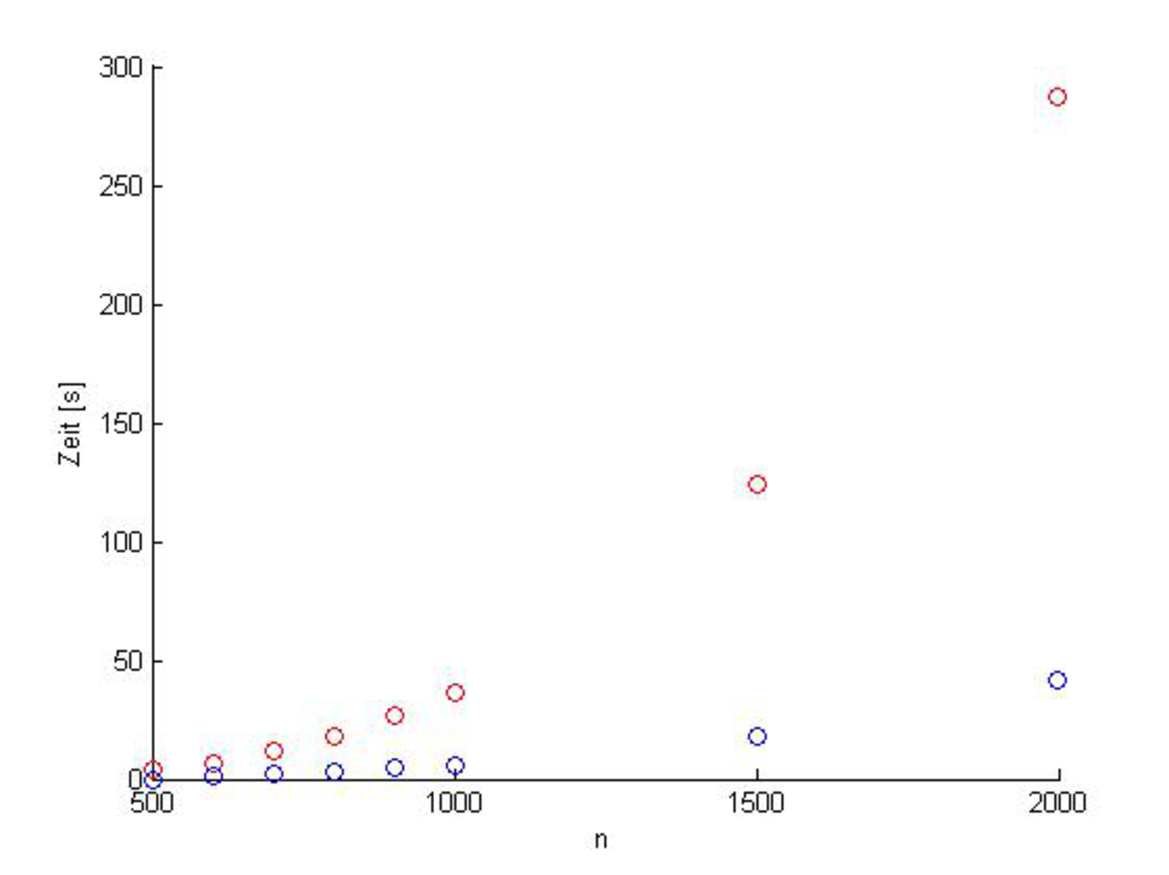
\includegraphics[width=8.5cm]{./innerepunkte/dickbesetztematrix.pdf}
\end{center}
\caption{Laufzeit f"ur voll besetzte Matrizen.
{\color{red}rot}: innere Punkte, {\color{blue} blau}: Simplex-Algorithmus
\label{innerpunkte:performance-vollbesetzt}}
\end{figure}

\begin{figure}
\begin{center}
  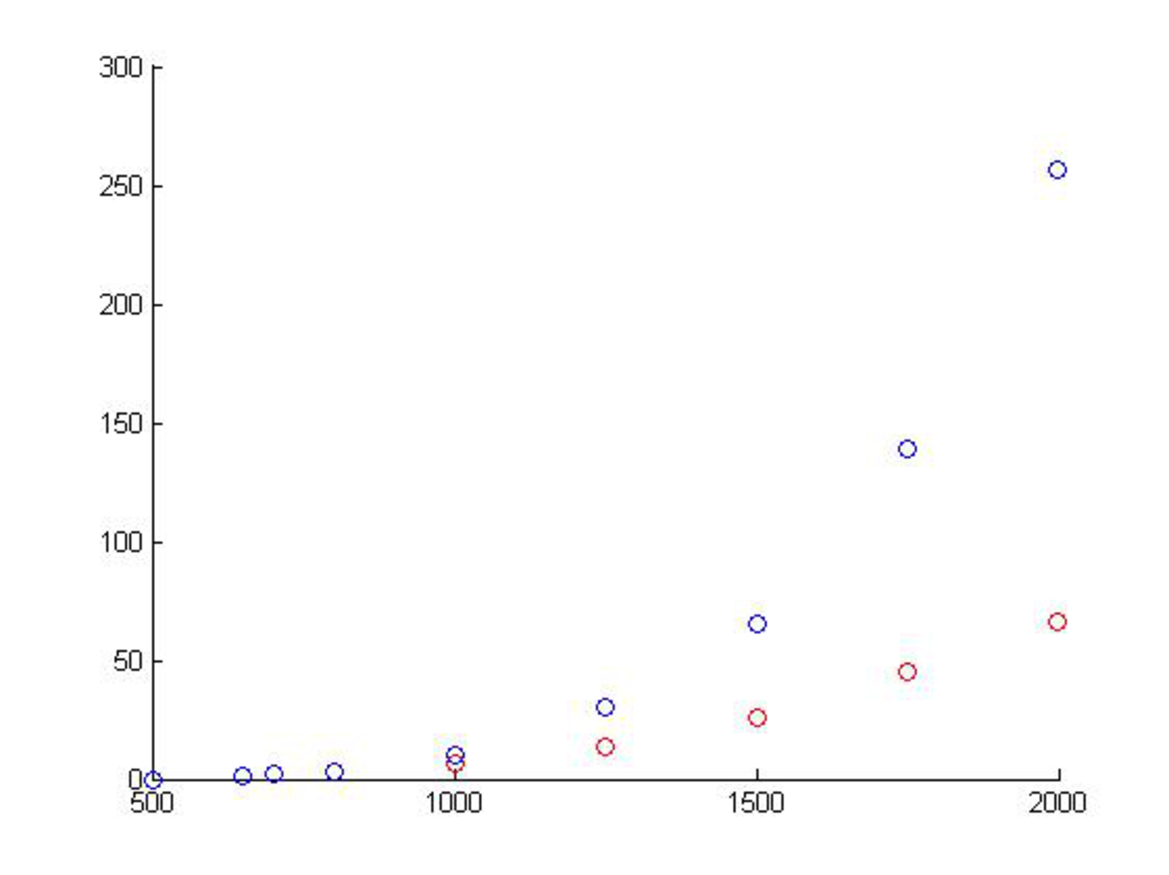
\includegraphics[width=8.5cm]{./innerepunkte/duennbesetztematrix.pdf}
\end{center}
\caption{Laufzeit f"ur d"unn besetzte Matrix.
{\color{red}rot}: innere Punkte, {\color{blue} blau}: Simplex-Algorithmus
\label{innerpunkte:performance-duennbesetzt}}
\end{figure}

%\end{figure}
%\begin{minipage}[t]{9.0cm}
%  \subsection{Zeit mit voll besetzter Matrix A}
%  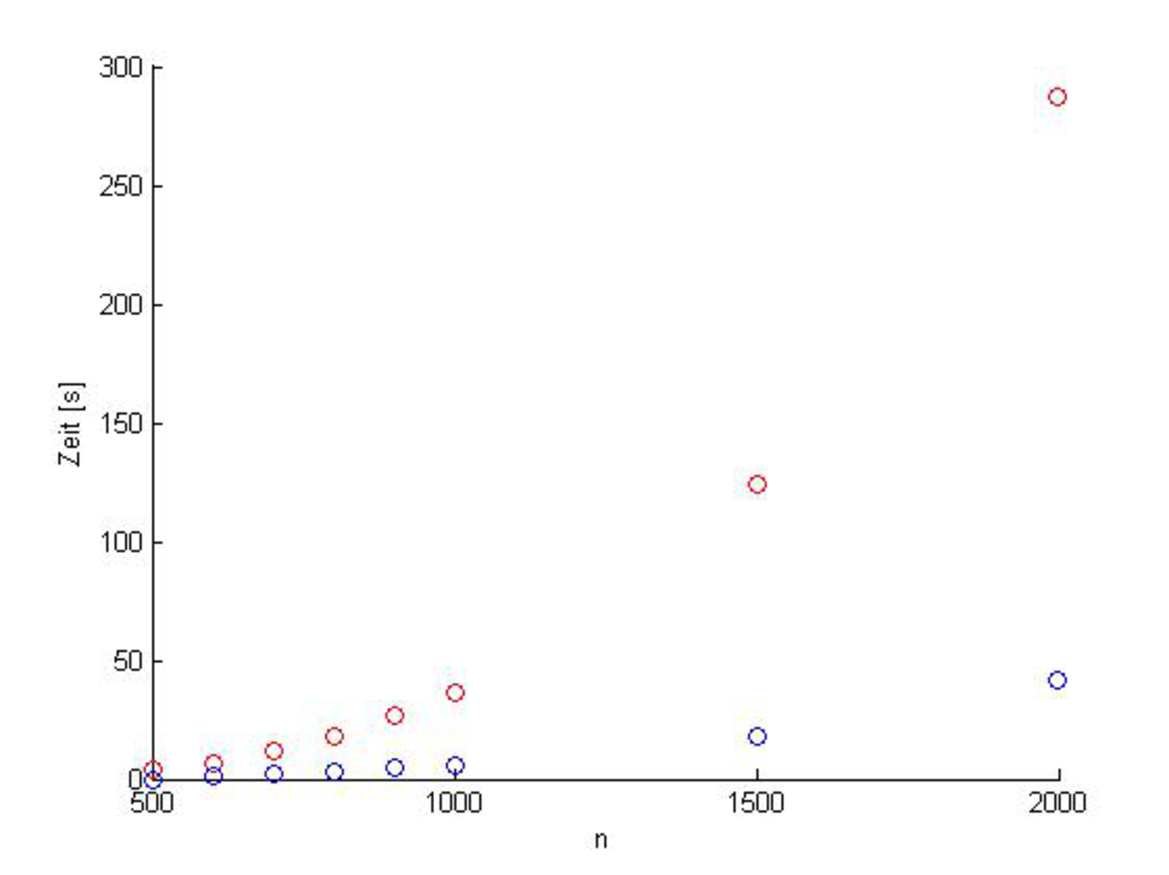
\includegraphics[width=8.5cm]{./innerepunkte/dickbesetztematrix.pdf}
%\end{minipage}
%\hspace{0.1cm}
%\begin{minipage}[t]{9.0cm}	
%	\subsection{Zeit mit d"unn besetzter Matrix A}
%	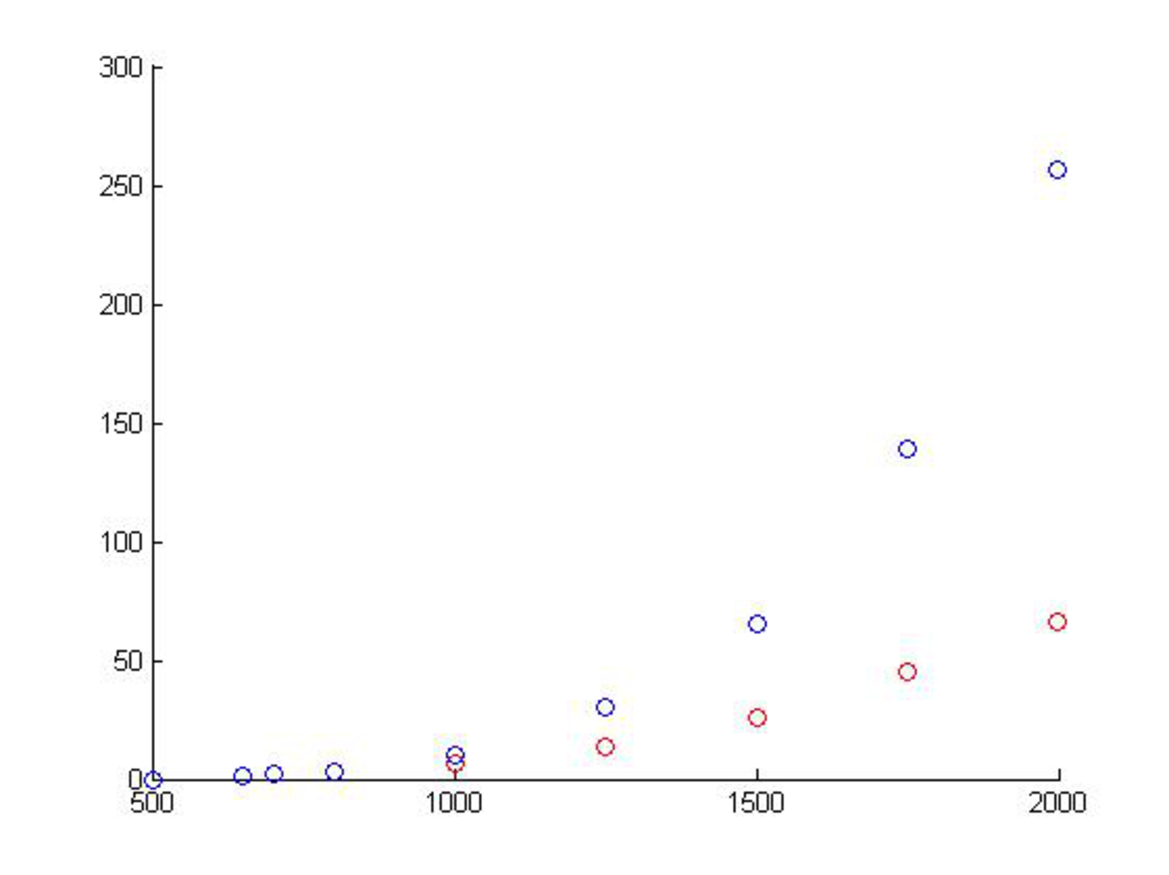
\includegraphics[width=8.5cm]{./innerepunkte/duennbesetztematrix.pdf}
%\end{minipage}



\section{Beispiel: Rosenbrock-Funktion}
An diesem Beispiel sieht man den verfolgten Pfad einer zweidimensionalen
Funktion. Es wurde nicht der Kurzschrittalgorithmus verwendet, da von
Punkt zu Punkt verschiedene Distanzen ben"utzt wurden. Man kann sich
das Prinzip f"ur andere Probleme auch in $3$ respektive $n$ Dimensionen
vorstellen.
\[
f(x_1, x_2) = 100 \cdot ((x_2+x_1^2)^2 + (1-x_1)^2)
\]
\begin{figure}
\begin{center}
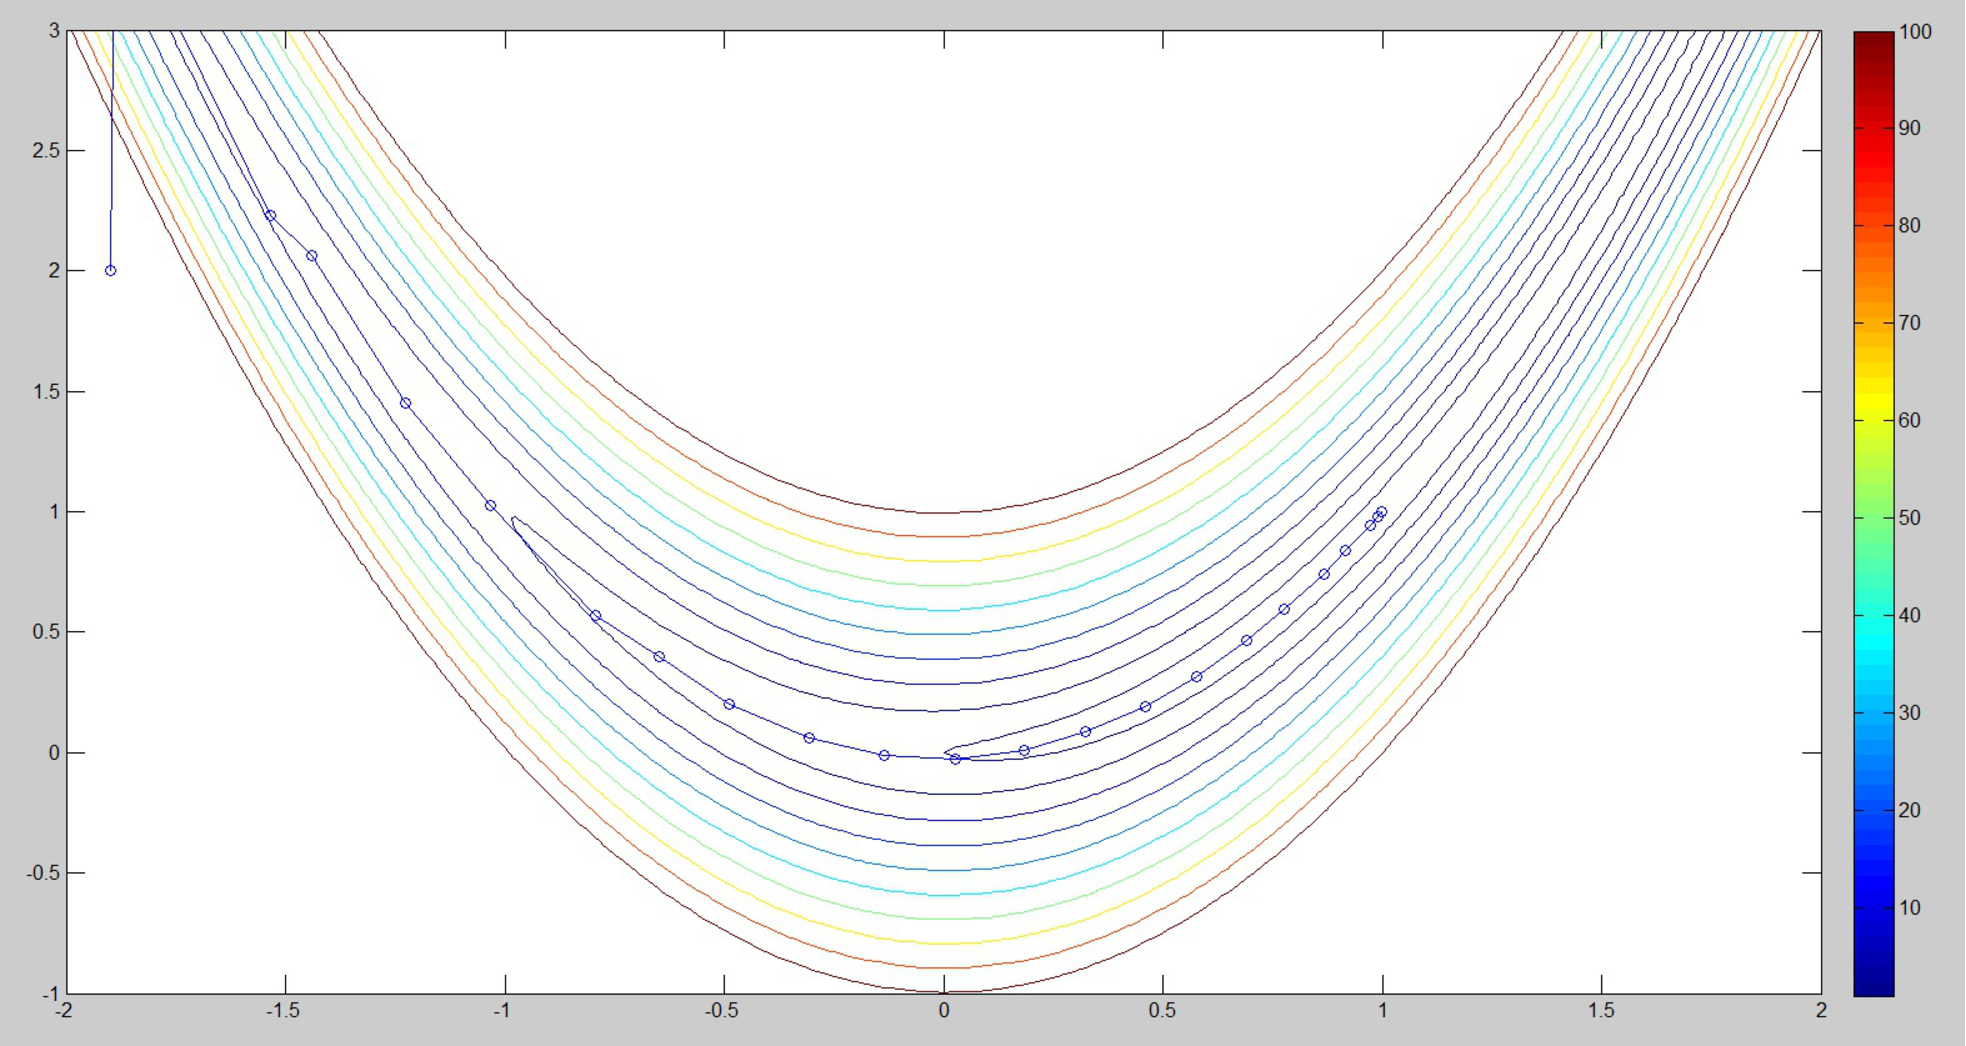
\includegraphics[width=\hsize]{./innerepunkte/Rosen.pdf}
\end{center}
\caption{Contour-Plot der Rosenbrock-Funktion sowie Weg des
Innere-Punkte-Verfahrens zum Minimum}
\end{figure}

\section{Beispielcode}
Der Beispielcode befindet sich im Github Repository im Verzeichnise
{\tt code/innerepunkte}.

\subsection{Code von Hand implementiert}
Diese Implementation verwendet keine Funktionen des GNU Linear Algebra
Toolkit, sie sollte mit jeder Version von Octave oder Matlab funktionieren.
Im Repository ist sie im File {\tt bsp2.m} enthalten.
\begin{lstlisting}[style=Matlab]
c =     [ 1,  6,  0,  3,  2]' % Zielfunktion, zu minimieren

A =     [ 2,  2,  0,  0,  0;  % Matrix mit Nebenbedingungen
         -1,  0,  2,  2,  0;
          0, -1, -1,  0,  2;
          0,  0,  0, -1, -1]

b =     [5, 0, 0, -5]'  % Vektor fuer Nebenbedingungen

e =     0.1*ones(5,1)   % Genauigkeitsgrenze (Toleranz)
I =     eye(5)	

n =     4
k =     1      % Iterationsvariable (Zaehler)
a =     1      % Kurzschrittalgorithmus: Schrittweite = 1

%-------------------% Schritt 1.)
x = 0.1*ones(5,1)   % Startvektor fuer primales Problem
y = 0.1*ones(4,1)   % Startvektor fuer duales Problem
s = 0.1*ones(5,1)   % Startvektor fuer Schlupfvariablen

%-------------------% Schritt 2.)
u = x' * s/n;

while u > 0.001         % Abbruchbedingung	

    S = diag(s);        % Diagonalmatrix, auf der Diagonalen
    X = diag(x);        % die Komponenten der Vektoren x, s

    % --------------% Schritt 3.)
    u = u * (1 - (1/6) / sqrt(n));  % neuer Straftermfaktor


    % --------------% Schritt 4.)
    dxdyds = [
              zeros(5), A',         I;
              A,        zeros(4),   zeros(4,5);
              S,        zeros(5,4), X
             ]  \  [
                     c - A' * y - s;
	             b - A * x;
                     u * e - S * X * e
                   ];


    % --------------% Schritt 5/6.)
    x = x + a * [ dxdyds(1),
                  dxdyds(2),
                  dxdyds(3),
                  dxdyds(4),
                  dxdyds(5)]';  % xneu = xalt + dx 
    y = y + a * [ dxdyds(6),
                  dxdyds(7),
                  dxdyds(8),
                  dxdyds(9)]';  % yneu = yalt + dy 
    s = s + a * [ dxdyds(10),
                  dxdyds(11),
                  dxdyds(12),
                  dxdyds(13),
                  dxdyds(14)]'; % sneu = salt + ds 
    
    k = k+1;  % Inkrementiere Variable k (Anzahl Durchlaeufe)

endwhile

k            % Ausgabe des k-ten Schritts
x            % Optimaler Punkt
\end{lstlisting}


\subsection{Code mit Hilfe von Octave-Funktion \textit{GLPK}}
Das GNU Linear Programming Toolkit implementiert das Innere-Punkte-Verfahren
und ist in GNU Octave "uber die Funktion {\tt glpk} zug"anglich
\cite{ip:glpk}.
Der folgende Code zeigt, wie die Funktion genutzt werden kann.
Im Repository ist dies das File {\tt bsp2octave.m}.

\begin{lstlisting}[style=Matlab]
c =     [ 1,  6,  0,  3,  2]'   % Zielfunktion, interpretieren
                                % als... (siehe Wert der
                                % Variablen s)

A =     [ 2,  2,  0,  0,  0;
         -1,  0,  2,  2,  0;
          0, -1, -1,  0,  2;
          0,  0,  0, -1, -1]

b =     [5, 0, 0, -5]'
lb=     zeros(5,1)   % lower bound (=0, falls keine
                     % Untergrenze angegeben)
ub=     []           % upper bound (=unendlich, falls keine
                     % Obergrenze angegeben)
ctype = "UUUU"       % U = Ungleichung mit Obergrenze
                     % (b enthaelt groesstmoegliche Werte)
vartype="CCCCC"      % C = Continuous Variable;
                     % I = Integer Variable;
s =     1            % -1 = Maximierungsproblem;
                     % 1 = Minimierungsproblem;

        
param.msglev = 3     % Parameter: Level of messages output by
                     % solver routines (1=no - 4=full)
param.itlim = 1000   % Parameter: Simplex max. Anzahl
                     % Iterationen
param.lpsolver =  2  % Parameter: 1=Simplex / 2=innerePunkte

          
[xopt, fopt, status, extra] = glpk (c, A, b, lb, ub, ctype, vartype, s, param);


status    % 150=innerPointMethod is undefined oder
          % 151=innerPointMethod is optimal
extra     % lambda=dual variables;
          % redcosts = reduced costs; 
          % time = time in seconds for LP/MIP problem; 
          % mem = memory used for LP/MIP in bytes

		
xopt      % Optimum, bester Punkt	
fopt      % Wert des Optimums / des besten Punktes
\end{lstlisting}

\printbibliography[heading=subbibliography]
\end{refsection}

%\section{Quellen}

%\url{http://de.wikipedia.org/wiki/Innere-Punkte-Verfahren}\\
%\url{http://www.gnu.org/software/octave/doc/interpreter/Linear-Programming.html}\\
%\url{http://www.ruhr-uni-bochum.de/num1/files/theses/da_tunc.pdf}\\
%\url{http://www.math.uni-hamburg.de/home/j.werner/kap4.pdf}\\
%\url{http://www-m1.ma.tum.de/m1old/personen/sulbrich/opt3}
